\chapter{Preliminaries}\label{ch:preliminaries}
This chapter presents the most fundamental and relevant theory that is necessary to understand the rest of the chapters in the report. Note that this does not include the theory behind Timed I/O Transition Systems, Timed Input/Output Automata, Implementations, Specifications and all the associated features: Refinement, Structural Composition and Logical Conjunction as it was already defined in \textcite{Jecdar:2019}.

\section{Refinement rules}\label{sec:refRules}
According to \textcite{David:2010}, "A notion of refinement allows to compare two specifications as well as to relate an implementation to a specification. Refinement should satisfy the following substitutability condition. If $P$ refines $Q$, then it should be possible to replace $Q$ with $P$ in every environment and obtain an equivalent system". This completely makes sense, since refinement follows three basic rules.

A specification $S = (St^S, s_0, \Sigma^S ,\rightarrow^S)$ refines a specification \\ $T = (St^T, t_0, \Sigma^T ,\rightarrow^T)$, written $S \leq T$, iff there exists a binary relation $R \subseteq St^S \times St^T$ containing ($s_0,\ t_0$) such that for each pair of states ($s,\ t) \in R$ we have:
\begin{itemize}
    \item whenever $t \xrightarrow{i?}^T t'$ for some $t' \in St^T$ then $s \xrightarrow{i?}^S s'$ and ($s',\ t') \in R$ for some $s' \in St^S$.
    \item whenever $s \xrightarrow{o!}^S s'$ for some $s' \in St^S$ then $t \xrightarrow{o!}^T t'$ and ($s',\ t') \in R$ for some $t' \in St^T$.
    \item whenever $s \xrightarrow{d}^S s'$ for $d \in \mathbb{R}_{\geq 0}$ then $t \xrightarrow{d}^T t'$ and ($s',\ t') \in R$ for some $t' \in St^T$.
\end{itemize}
In the rest of the report we will refer to these rules as refinement input, refinement output and refinement delay rules respectively.

\section{Additional outputs on the left side}\label{sec:addOutputsLeft}
The definition of refinement states that the set of actions belonging to the transition system on the left side should be identical to the one on the right side. However, this restrains the transition systems, which greatly reduces possibilities such as having the composition of multiple components on the left side.

\ecdar does not seem to introduce such restrictions, thus there can be scenarios in which it does not perform in accordance with the theory.

Our implementation tries to make a compromise between the theory and \ecdar, namely by allowing the left side to have more output actions. This is particularly useful when the left side consists of a composition of multiple automata which synchronize together on certain actions that we do not necessarily require to match on the right side. In this case, we allow the right side not to have those outputs and instead treat it as if those outputs are ignored, by adding self-loops for all missing outputs.

This newly introduced signature check comes as a precondition of the refinement. If either the set of output actions of the left side differs from the one on the right or the left side does not contain all the input actions of the right side, then the refinement check fails immediately, without exploring the state space. If the preconditions are met, only then can the check be performed.

\section{The left side is the driving side}\label{sec:leftDominant}
Probably the most important observation that was made was that the left side is the dominant side in the refinement. Without this knowledge it would be impossible to make the refinement work properly. The right side of the refinement can be the driver side only for the inputs, while the left side will dominate in all other cases. Considering the fact that two out of three rules are in favor of the left side, as well as the fact mentioned in Section \ref{sec:addOutputsLeft}, which allows more outputs on the left side, one may call the left side being the "dominant" one.

\section{Refinement feature issues}
Our implementation of the refinement feature appeared to be complete and correct, as all our tests were passing and we had significantly high code coverage. However, after some in-depth analysis we discovered that in some cases the size of the explored state-space was unusually small. At this point, we started investigating the possible causes of this problem and we identified several inconsistencies and aspects that we had not been aware of to that point, which are documented in Chapter \ref{ch:inconst}.

Further, we present a selection of concepts that we introduced in an attempt to achieve a correct implementation of the refinement feature.

\section{DBM Raw Values} \label{sec:raw-values}
The knowledge that will be required to understand some of the practical concepts from Chapter \ref{ch:concepts} includes the exact understanding of how the zones are stored. As described in \textcite{Jecdar:2019}, zones in \jecdar are represented with the Difference Bound Matrix(DBM) data structure, using the DBM Library implementation (\textcite{dbm-library-web}). Even though one may constrain the clocks of a zone with the integer values of the bounds obtained from such constraints as guards or updates, the \textcite{dbm-manual} documentation of the DBM Library states that each clock constraint is internally encoded into a \textbf{raw\_t} type that is used for all DBM related computations. In the rest of the report, we refer to these encoded constraints as "raw" values. The actual bounds are referred to as "actual" values or bounds. 

\begin{table}
\centering
\begin{tabular}{| c | c || c | c |}
\hline
Bound & Raw & Bound & Raw \\
\hline
$\leq -1$ & -1 &$< 0$     & 0  \\
$< -1   $ & -2 & $\leq 0$ & 1  \\
$\leq -2$ & -3 &$< 1$     & 2  \\
$< -2   $ & -4 & $\leq 1$ & 3  \\
$\leq -3$ & -5 &$< 2$     & 4  \\
$< -3   $ & -6 & $\leq 2$ & 5  \\
$\leq -4$ & -7 &$< 3$     & 6  \\
$< -4   $ & -8 & $\leq 3$ & 7  \\
$\leq -5$ & -9 &$< 4$     & 8  \\
$< -5   $ & -10 & $\leq 4$ & 9  \\
$\leq ...$ & ... & $< ...$ & ...  \\
\hline
\end{tabular}
\caption{Raw values of DBM}
    \label{tbl:raw-values}
\end{table}

The main purpose of the encoding is to be able to tell the difference between the different strictness of a given bound or constraint (ex. $\leq 5$ and $< 5$). Note that the constraints defining the lower bound of an interval, such as $x \geq 3$, will end up being stored as negative constraints (-3) due to having to flip the inequality sign to match the $<$ or $\leq$ inequality sign required by the DBM. Table \ref{tbl:raw-values} demonstrates the correspondence between a constraint and the raw value associated with it and is just a small excerpt of bounds from the huge set of possible values. Listing \ref{lst:bound2Raw} provides with a formula used to calculate raw values from actual ones. The understanding of this relationship will further help us to understand the origin of various problems related to concepts that are yet to be explained.

\begin{lstlisting}[caption = {Formula to calculate raw values from actual values}, label = {lst:bound2Raw}, mathescape=true]
if(sign == '<') raw = actual*2
if(sign == '$\leq$') raw = actual*2+1
\end{lstlisting}

\section{Arrival, invariant and guard zones}
In subsequent chapters of the report some of the figures of automata will contain zones generated at different times during the exploration of the state space. Each of these zones will be equally important and syntactically equivalent to the rest, however the difference in their underlying semantics will strongly influence their purpose and use in concepts. In simple words, each of these zones will contain different information related to guards, invariants and resets. In this section we introduce notation for three types of zones: \textbf{arrival zone, invariant zone} and \textbf{guard zone}.

Note that for simplicity and readability reasons we choose to represent the zones from the figures as intervals instead. However, if necessary in further examples these zones will be represented as zones instead. Additionally, only necessary information (zones, intervals, etc.) will be shown in figures in later sections to ensure readability.
 
Figure \ref{fig:three-zones} shows an example of an automaton with one clock \textbf{x} and is enriched with all three kinds of zones. The zones shown above the location (mostly top-left) are referred to, in this report, as \textit{arrival zones}. They show what values clock \textbf{x} can evaluate to when one arrives at a certain location. Since location \textbf{id0} is an initial location, it comes naturally that clock \textbf{x} can only have one possible clock valuation - $0$.

\begin{figure}
\centering
\begin{tikzpicture}[thick,scale=0.9, every node/.style={scale=0.9}]
    \node[anchor=south west,inner sep=0] (image) at (0,0)
    {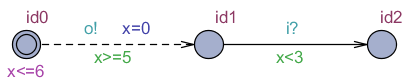
\includegraphics{figures/three-zones.png}};
    \begin{scope}[x={(image.south east)},y={(image.north west)}]
        \node[font=\Large] at (-0.02,0.8) {$\bm{x[0;0 ]}$};
        \node[font=\Large] at (0.06,-0.15) {$\bm{x[0;6]}$};
        \node[font=\Large] at (0.45,0.8) {$\bm{x[0;0 ]}$};
        \node[font=\Large] at (0.28,0) {$\bm{x[5;6 ]}$};
        \node[font=\Large] at (0.5,0) {$\bm{x[0;\infty )}$};
        \node[font=\Large] at (0.7,0) {$\bm{x[0;3 )}$};
        \node[font=\Large] at (0.83,0.8) {$\bm{x[0;3 )}$};
        \node[font=\Large] at (0.92,0) {$\bm{x[0;\infty )}$};
    \end{scope}
\end{tikzpicture}
\caption{Demonstration of arrival, invariant and guard zones} \label{fig:three-zones}
\end{figure}

Zones referred to as \textit{invariant zones} are the ones normally depicted below the location. As a rule, the invariant zone is derived from the arrival zone by performing the delay operation followed by the application of all invariants belonging to the corresponding location. The invariant zone shown under location \textbf{id0} provides information about how long one can stay in the same location by delaying (up to \textbf{6} time units).
 
The last zone to be introduced - \textit{guard zone}, refers to the zone representing all possible clock valuations during which an edge can be taken. The guard zone is derived from the invariant zone by applying all guards associated with that edge. For example, the edge from \textbf{id0} to \textbf{id1} can only be taken with clock \textbf{x} valuations belonging to an interval from \textbf{5} to \textbf{6}.
 
The arrival zone of the target of an edge is then derived from the guard zone of that edge by applying all associated resets. Therefore, the arrival zone at location \textbf{id1} is shaped by the reset on the edge leading to that location, whereas the arrival zone at location \textbf{id2} is equivalent to the guard zone of the edge leading to that location due to the absence of resets.

Even though many of these zones may seem obvious and intuitively derivable from the image of an automaton, in the code of \jecdar these zones are the only source of information during the computation of Refinement, Composition and Conjunction and therefore all of the further algorithms operate with the presented zones.